%%%%%%%%%%%%%%%%%%%%%%%%%%%%%%%%%%%%%%%%%%%%%%%%%%%%%%%%%%%%%%%%%%%%%%%%%%%
% Juan Manuel Perez Rua
%%%%%%%%%%%%%%%%%%%%%%%%%%%%%%%%%%%%%%%%%%%%%%%%%%%%%%%%%%%%%%%%%%%%%%%%%%%

\chapter{Object Flow Pipeline} \label{chap:core}

\section{Algorithm description}
\label{sec:desc}

The Fig. \ref{figurelabel_sys} shows a simplified block diagram of the proposed system. Two details are important, 
the use of the tracker window to initialize a segmentation procedure, and the use of this segmentation over the tracked window 
to perform a more precise motion flow computation in the interest pixels. The dotted line represents the possible interaction 
between precise flow information and the next tracker state. For instance, the current object flow can work as direction hint, and 
the segmentation information can be used to improve the sampling process of the learning stage in several trackers by detection methods \cite{c22}, and 
thus the tracker and motion flow algorithm can work for mutual enhancement.

   \begin{figure}[thpb]
      \centering
      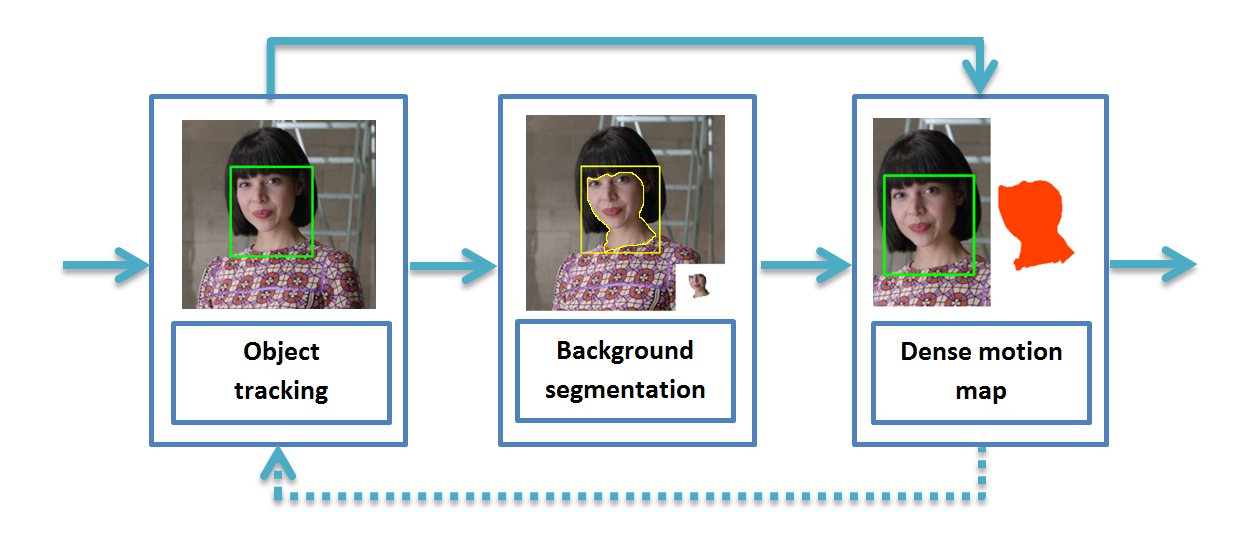
\includegraphics[width=1.00\textwidth]{../images/system.png}
      \caption{Block diagram of the proposed pipeline.}
      \label{figurelabel_sys}
   \end{figure}

The first step in the object flow pipeline can be selected according to specific need for a given application. We prefer, in general, tracking-by-detection methods 
like $Struck$ \cite{c22} or $MIL$ \cite{c23}, but other approaches could be followed. In the second place, for the object segmentation in video we propose the use 
of labelled background regions through the concept of superpixel flow, which is explained in the next section.

%%%%%%%%%%%%%%%%%%%%%%%%%%%%%%%%%%%%%%%%%%%%%%%%%%%%%%%%%%%%%%%%%%%%%%%%%%%
% Juan Manuel Perez Rua
%%%%%%%%%%%%%%%%%%%%%%%%%%%%%%%%%%%%%%%%%%%%%%%%%%%%%%%%%%%%%%%%%%%%%%%%%%%

\section{Superpixel flow} \label{sec:suppix}

\subsection{Problem definition}
Superpixels and over segmentation techniques became a widely used pre-processing 
stage for a large number of machine vision applications, after the
original concept was introduced \cite{c1}. Superpixels are traditionally used as 
performance booster for several other techniques. However, it is still mostly related to
single frame processing \cite{c1}\cite{c10}\cite{c11}. In the search for
consistency in superpixel labelling through video, some authors have proposed different 
techniques, which go from simple extension to supervoxels\cite{c9}\cite{c11},
to more complicated approaches \cite{c8}. These approaches, nonetheless, usually require a 
global processing and knowledge of all (or several of) the video frames beforehand. 

As a preprocessing step in the object flow pipeline, we propose a superpixel matching technique which assumes a flow-like behaviour in the image 
sequences (natural video), which can be used to track superpixels. 
Some previous work have been done towards a
superpixel based image comparison using the Earth Mover's Distance, by taking superpixels 
as bins of a global histogram \cite{c2}. The label propagation or superpixel flow can be
achieved with this technique as a by-product, by selecting the superpixel in the second frame that 
maximize the EMD flow from each superpixel in the first frame.
By taking into account superpixels computed separately in images, so the video process can be 
performed with only two frames at a time, we move towards a more time efficient approach. 
This matching, however, has to comply with a set of constraints. 
Firstly, two correspondent superpixels should be similar in terms of some appearance
feature, which most likely depends on the way the superpixelization was performed (color, texture,
shape). Also, the superpixel flow  should maintain certain global regularity (at least for
superpixels that belong to the same object). In this sense, it seems
natural that the problem of superpixel flow could be solved with a discrete energy minimization
procedure. 
If the size compactness of the superpixels is maintained,  it actually seems to 
share some of the properties of the optical flow problem, with the difference that the
smoothness is usually a very strong constraint for the last one. 
The strength of this smoothness prior relies not only in the nature of the problem, but also
because it gives better cues towards an easier-to-minimize global approach.

The objective of the superpixel flow is therefore to find the best labeling $l$ for every superpixel $p$
(with $l_p \in {0,1,...N-1}$) between a pair of frames ($I_{0}$,$I_{1}$), but holding a flow-like behavior.

Thus, the superpixelization should maintain certain size homegenity within a single frame. Some super
pixel techniques can cope with this requirement \cite{c9}\cite{c10}. For the experiments presented 
in this work, the SLIC method \cite{c9} is prefered, because it usually gives
good results in terms of homegenity of the superpixelization across the sequence. 
The proposed steps to solve the propagation problem assume this requirement is hold. 
For other kind of the techniques, other approaches should be followed.

%\addtolength{\textheight}{-3cm}   % This command serves to balance the column lengths
%%%%%%%%%%%%%%%%%%%%%%%%%%%%%%%%%%%%%%%%%%%%%%%%%%%%%%%%%%%%%%%%%%%%%%%%%%%%%%%%

\subsection{Energy Formulation}

Inspired by a large number of optical flow and stereo techniques \cite{c7}\cite{c12}\cite{c13}, 
the superpixel flow can be modeled with a pairwise Markov Random Field. If
the matching is performed with MAP inference, its posterior probability is: 

\begin{equation}
P(l|I_0,I_1) = \displaystyle \prod_{p \in \Omega} \mathrm{e}^{-D_p(l_p;I_0,I_1)} 
\prod_{p,q \in \mathcal{N}_r} \mathrm{e}^{-S_{p,q}(l_p;l_q)} ,
\label{eq_prob}
\end{equation}

With $l$ the set of labels of the super pixels in $I_0$,
that match with those in $I_1$.
$ \mathcal{N}_r $ is a neighbourhood of the
superpixel $p$ containing all the superpixels which are inside a circle of radius $r$ with center in $p_c$. This neighbourhood defines its adjacency. 
Given this posterior probability, the equivalent energy function can be directly obtained
by extracting the negative logarithm of the posterior,

\begin{equation}
E(l) = \displaystyle \sum_{p \in \Omega} D_p(l_p;I_0,I_1) +
\sum_{p,q \in \mathcal{N}_r} S_{p,q}(l_p,l_q)
\label{eq_energy}
\end{equation}

The terms $D$, and $S$ in (\ref{eq_energy}) stand for data term and spatial smoothness terms as they
are popularly known in the MRF literature. The first one determines how accurate is the labelling in terms
of consistency of the measured data (color, shape, etc.). In the classical optical flow formulation of this equation,
the data term corresponds to the pixel brightness conservation\cite{c7}\cite{c5}. However, as superpixels are a set
of similar (or somehow homogeneous) pixels, an adequate appearance based feature can be a low dimensional
color histogram with $N$ bins. So $D$ can be written more precisely as the Hellinger distance between the histograms:

\begin{equation}
D_p(l_p;I_0,I_1) = \sqrt{ 1 - \frac{1}{\sqrt{\bar{h}(p)\bar{h}(p')N^2} } \sum_{i}\sqrt{h_{i}(p)h_{i}(p')} }
\label{eq_Dp}
\end{equation}

Where $h(p)$ and $h(p')$ are the histograms of the superpixel $p$ and its correspondent superpixel in the
second frame $I_1$. 
Note that the low dimensional histogram ($N=2, N=3$) gives certain robustness against noise,
and slowly changing colors between frames. 

On the other hand, the spatial term is a penalty function for horizontal
and vertical changes of the vectors that have origin in the centroid of the superpixel of the first frame and
end in the centroid of the superpixel of the second frame.

\begin{equation}
S_{p,q}(l_p, l_q) = \lambda(p)
  \sqrt{\frac{|u_{p_c}-u_{q_c}|}{\|p_c-q_c\|}+ \frac{|v_{p_c}-v_{q_c}|}{\|p_c-q_c\|}}
\label{eq_Spq}
\end{equation}
\begin{center}
 where, $ \lambda(p) = (1 + \rho(h(p),h(q)))^2 $ \\
\end{center}

In (\ref{eq_Spq}) the operator $\rho$ is the Hellinger distance as used in the
data term (\ref{eq_Dp}). The histogram distance is nonetheless computed between superpixels $p$ and $q$, 
which belong to the same neighbourhood. The superpixels centroids are noted as $q_c$ and $p_c$, 
and $u$ and $v$ are the horizontal and vertical changes between centroids.
This term is usual in the MRF formulation and has a smoothing effect in superpixels that belong to the
same object. It has to be observed that when two close superpixels are different, thus, more probable to
belong to different objects within the image, the term $\lambda$ allows them to have
matches that do not hold the smoothness prior with the same strength. 
It has to be noted that the proposed energy function is highly non-convex.

\subsection{Energy Minimization}

A fair amount of work has been dedicated to discrete optimization techniques in computer vision,
leading to well-defined and widely tested approaches to solve pairwise MRF\cite{c3}\cite{c4}.
However, some of the approaches restrict the construction of the spatial term, and/or enforce
limitations in the number of labels \cite{c3}.
Because of the high amount of possible labels for  each superpixel in the proposed approach, the use of the
Fusion Moves \cite{c7} technique seems to be well suited.
This algorithm employs the Quadratic Pseudo-Boolean Optimization (QPBO), to combine
incremental sets of proposal labellings, resulting in a semi-globally-optimal solution \cite{c4}.
Thus, the minimization starts by proposing a set of possible solutions, and iteratively merges them with
the QPBO technique. 

The candidate solutions depend on the problem to be solved. 
For example, in stereo superpixel matching, some assumptions related to the cameras 
layout can be made to generate solutions. In a more generic sense, other assumptions can be made towards 
candidate generation. 
The Quadratic Pseudo-Boolean Optimization (QPBO) \cite{c3}\cite{c4} is used to minimize the proposed energy function, 
by merging a set of candidate matches for every superpixel in the first frame.
For instance, for a given superpixel in the initial frame, the corresponding 
matching would be the most similar one in terms of color, shape, or the spatial distance. More candidate solutions can be added by defining a
neighbourhood in the second frame and select random pairs from every neighbourhood of every superpixel
in the first frame. This is suitable for problems where the images are extracted from the same video
sequence. 
To speed-up the minimization procedure, the QBPO properties can be exploited. For instance, the fusion of the
proposed solutions is always guaranteed to be of lowest or equal energy than the two proposals. Thus, one could
split the fusion procedure in several cores and build a hierarchical chain as fusions of proposal are subsequently fused.

   \begin{figure}[thpb]
      \centering
      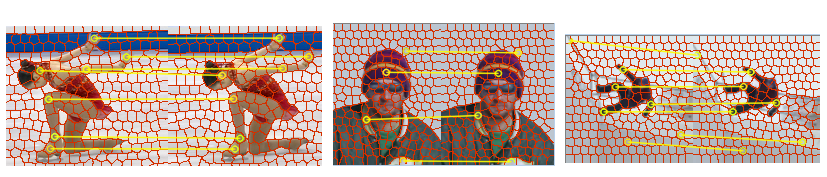
\includegraphics[width=1.00\textwidth]{../images/matches.png}
      \caption{The yellow lines show selected superpixel
		matching between pairs of consecutive frames in a video
		with the proposed method. The video frames go from right
		to left.}
      \label{figurelabel_matches}
   \end{figure}

\subsection{Matching Results}
   \begin{figure}[thpb]
      \centering
      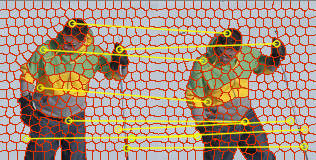
\includegraphics[width=0.70\textwidth]{../images/matches_snowshoes.png}
      \caption{The yellow lines show selected superpixel
		matching between a pair of distant frames in the Snow Shoes sequence.}
      \label{figurelabel_matchessnow}
   \end{figure}   
	\setlength{\belowcaptionskip}{-10pt}
	
The Fig. \ref{figurelabel_matches} shows some examples of superpixel matching between subsequent frames with the presented method. 
It can be seen that the matching performs well even in difficult cases, like the hands in the top row. It has to be noted
as well that even in superpixels where there is a lack of texture, there is correct matching. This seems to be
the effect of enforcing the regularization between superpixels that are close, but are also similar to
each other.
 
Moreover, unlike most of the optical flow methods, superpixel flow extends 
 naturally for more distant frames. 
The Fig. \ref{figurelabel_matchessnow} shows
 results for large separations between frames, without tweaking or adjusting any parameters. 
For this case, however, the matches in the texture-less part of the scene
 are mostly invalids. Though this is expected because of the aperture problem and
 heavy occlusions.

%%%%%%%%%%%%%%%%%%%%%%%%%%%%%%%%%%%%%%%%%%%%%%%%%%%%%%%%%%%%%%%%%%%%%%%%%%%
% Juan Manuel Perez Rua
%%%%%%%%%%%%%%%%%%%%%%%%%%%%%%%%%%%%%%%%%%%%%%%%%%%%%%%%%%%%%%%%%%%%%%%%%%%

\section{Background regions tracking and segmentation}
\label{sec:segm}
The algorithm proposed in \cite{c18}, offers a good deal in terms of
background-foreground separation from user interaction. A technique like this, however,
performs very well in still images, but it may not be well adapted for sequential videos. 
Extensions to this method, like the GrabCut algorithm \cite{c14}, work by implementing an iterative graph-cut based 
minimization to separate regions according to appearance information from a loosely drawn rectangle around the object, and small user-interaction-based hints. 
Given the tracker state for every frame, the minimization procedure of the methods in \cite{c18} and \cite{c14} could be extended to video. However, 
a lot of details in the segmentation contour may be lose if no fine hints are given.
These hints usually depend on on-the-fly supervised methods. However, this need could be minimized in videos, given the extra information that offers the dynamics of the sequence.
Some authors had approached the graph-cut based segmentation techniques in sequential
videos to propagate a consistent segmentation \cite{c15}. However, some more work on reducing user interaction given the extra flow-like information
that video sequences offer is still needed.
Determining the spatial support of the object in a given frame benefits from the output of the tracker. Appearance cues alone, learned inside and outside the tracking window 
can result in a misleading modelling of the foreground and the background. In contrast, we propose to perform foreground-background segmentation by tracking 
background pixels surrounding the target, thanks to the tracker output. Thus, the pixels that are initially outside the tracker window, 
are followed through the sequence and as long as they enter the tracked region, they can be safely labelled as background. 
This idea can be observed in the Fig.  \ref{figurelabel_entering}, 
where the object window given by the tracker (green) loosely separates the foreground from the background. Points outside the tracker (blue) are labelled as background in previous frames, and as they enter the tracker window (red points), they can be used to improve the modelling  of the foreground and the background. 
The red window is used to save computational power by avoiding to track points that are too far from the interest object.

   \begin{figure}[thpb]
      \centering
      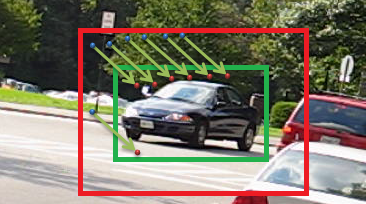
\includegraphics[height=0.285\textheight]{../images/tracking_points.png}
      \caption{Example image of points entering a tracking region (green) due to object motion in a video sequence.}
      \label{figurelabel_entering}
   \end{figure}
\setlength{\belowcaptionskip}{-10pt}

   \begin{figure}[thpb]
      \centering
      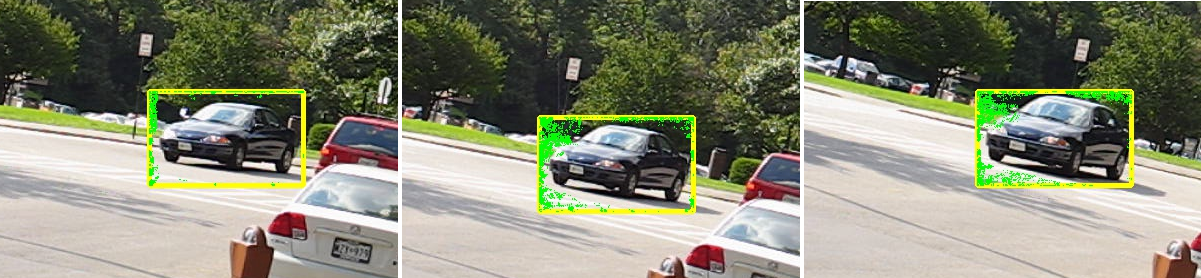
\includegraphics[width=1\textwidth]{../images/pointTr.png}
      \caption{Point tracking using an optical flow method.}
      \label{pointtr}
   \end{figure}


This idea can be applied in several levels in a video sequence. The first method to develop such an algorithm is to do it in the pixel level. The Fig. \ref{pointtr} shows some results by applying 
a dense optical flow technique (Fast Block Matching) in an external window. However, as it can appreciated, the results are rather sparse and after some time, the regularization of the 
optical flow method leads to some of the points being wrongly tracked inside the object boundaries. Both problems, sparsity and tracking errors due to drift and regularization, can be 
overcome by implementing the same idea, but in the superpixel level.
To save computational power, the tracked superpixels are 
limited to the ones that fall inside a control region (red box in the Fig.  \ref{figurelabel_entering}). 

Normally, after several frames, 
the labelled superpixels will almost completely cover the unwanted areas in a dynamic scene. We call this process background segments tracking and the process is summarized in the 
Algorithm \ref{algo1}.  The Fig. \ref{figurelabel_spflow} shows this idea in a real scenario. From left to right, initially the superpixels with 
elements outside the bounding box are labelled as background (green), then, as the sequence changes, the labelled superpixels flow inside the window, giving hints for the model initialization in the background-foreground separation algorithm.

\begin{algorithm}[ht]
\caption{Background regions tracking between a frames A and B}
\label{algo1}
\begin{algorithmic}
\REQUIRE list: $superpixelsA, superpixelsB$, rect: $trackerA, trackerB$, vector: $prev\_labels$

\STATE vector: $new\_labels$
\STATE $computeSuperPixelFlow()$
\FORALL{$superpixel \in superpixelsA$}
    \STATE $matches[superpixel] = getMatchesFromFlow(superpixel)$

	\COMMENT{ Check is previously labelled superpixels fall inside $trackerB$ }
	\IF{$superpixel \in prev\_labels$}
		\STATE $matchAB = superpixelsB[ matches[superpixel] ]$
    		\IF{$matchAB \in trackerB$} 
    			\STATE $new\_labels.push\_back( matchAB )$
    		\ENDIF
	\ENDIF 

	\COMMENT{ Check is new labelled superpixels fall inside $trackerB$ }    
    \IF{$superpixel \notin trackerA$} 
    	    \STATE $matchAB = superpixelsB[ matches[superpixel] ]$
    		\IF{$matchAB \in trackerB$} 
    			\STATE $new\_labels.push\_back( matchAB )$
    		\ENDIF
    	\ENDIF
\ENDFOR

\RETURN $new\_labels$
\end{algorithmic}
\end{algorithm}

At this point, some generic segmentation technique can be connected to the pipeline to refine the segmentation (e.g. region growing). However, graph based segmentation methods are preferred (\cite{c18}\cite{c15}) because the usual user interaction can be replaced by the tracked background regions, and the algorithms are faster and more robust.

   \begin{figure}[thpb]
      \centering
      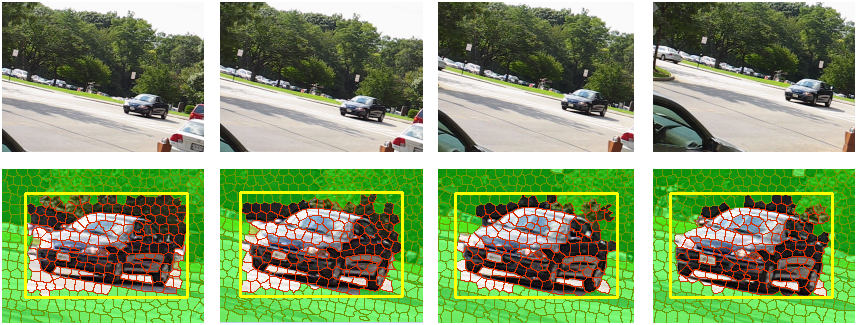
\includegraphics[width=1\textwidth]{../images/suppixflow2.png}
      \caption{Background segments automatic labelling and propagation, the flow goes from left to right.}
      \label{figurelabel_spflow}
   \end{figure}

\subsection{Segmentation results}

Fig. \ref{figurelabel_walking} shows the results for an image sequence where the interest object is the head of a person.
The head tracker and the superpixel flow provide information for better background-foreground separation. The
background-foreground models are updated as the frames go on, giving more robustness for sequential
propagation of the segmentation. The method is tested in the Walking Couple sequence, by allowing only a small amount of iterations in the
graph based segmentation. Observe how the contour in the man's head is correctly delineated when
another person's head occludes part of it. In this case, the superpixels that belong to the woman’s face
were correctly propagated and thus, labelled as background. Its also impressive that the segmentation process recovers after a heavy occlusion.
In this case, the fact that the tracker is also robust to the occlusion is a key factor that help the system maintain a correct segmentation through such a difficult 
case.

   \begin{figure}[thpb]
      \centering
      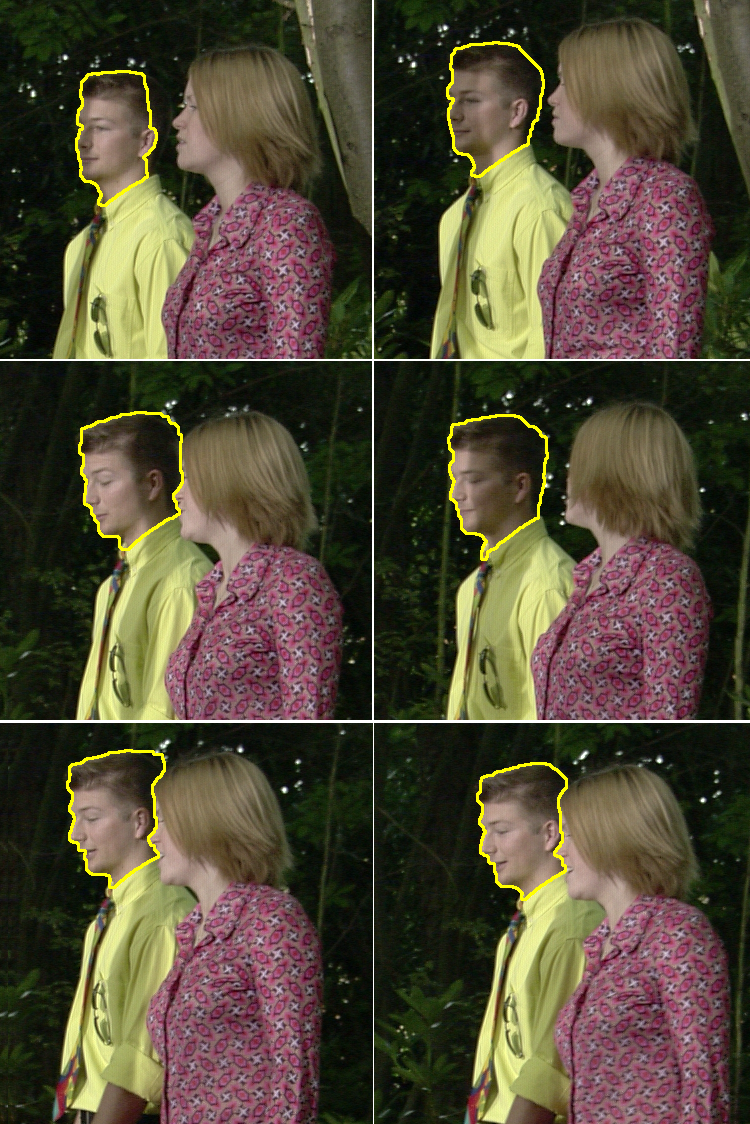
\includegraphics[width=1.0\textwidth]{../images/Sequence.png}
      \caption{Segmentation through the sequence “Walking
	       Couple” (Yellow contour) initialized in the man’s head. The yellow box correspond to the tracker output.
	        The labelled background superpixel are not shown for clarity.}
      \label{figurelabel_walking}
   \end{figure}

In order to understand the effect of including superpixel propagation in a video sequence for object
segmentation, some results are shown in the Fig. \ref{figurelabel_comp}. For these experiments only one iteration is
allowed in the graph-cut based methods. The top row frames (Fig. \ref{figurelabel_comp}) were initialized only with the tracker, 
and the bottom row was initialized with the superpixel tracking technique. 
Observe that in general, the contour delineated is usually better in terms of precision and
stability for the later one. Complete segmentation results can be observed in the Appendix \ref{app:seg}.

   \begin{figure}[thp]
      \centering
      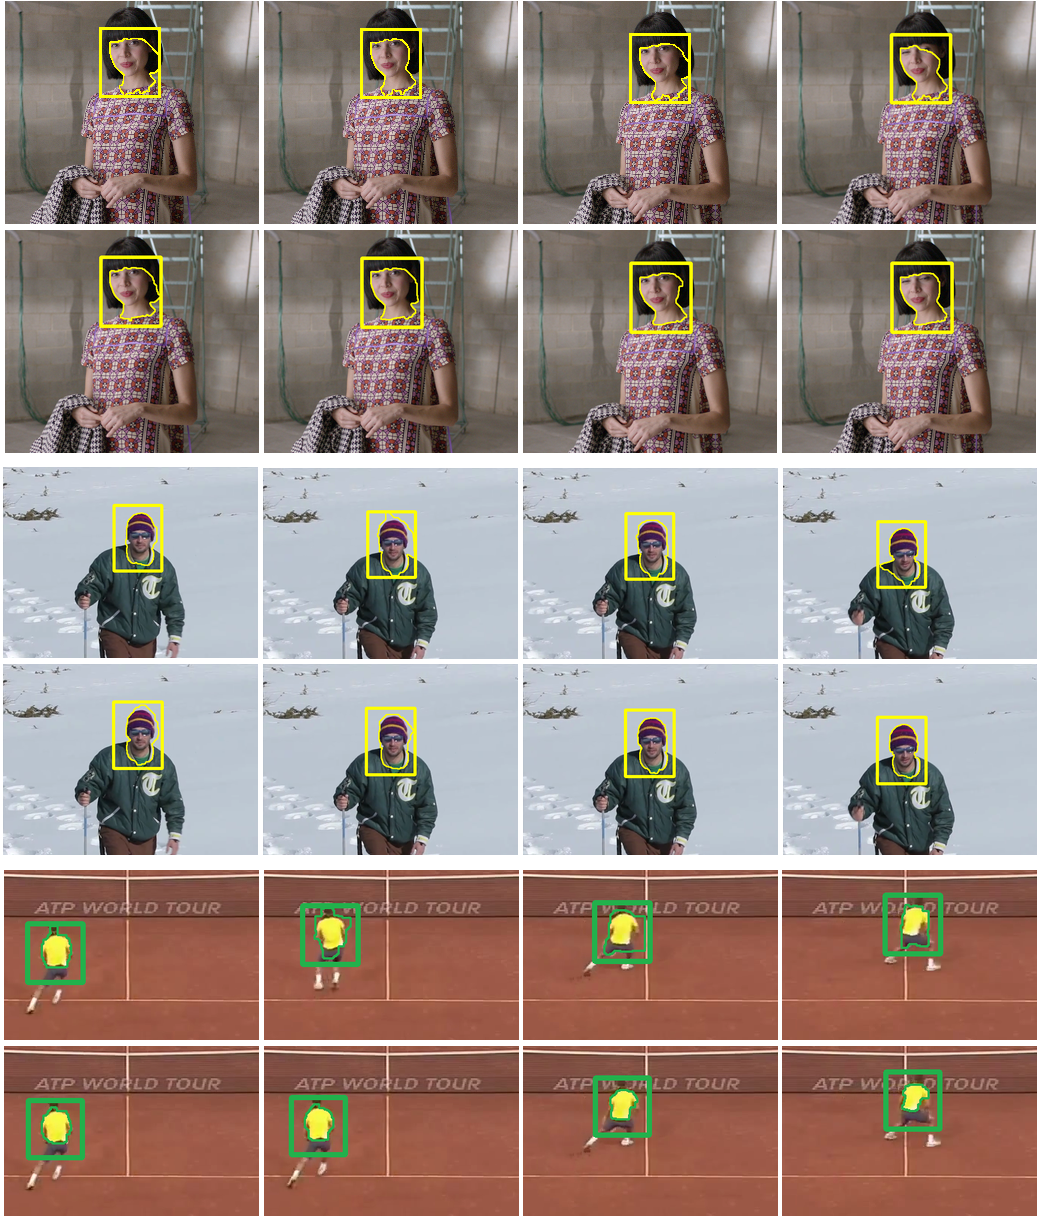
\includegraphics[width=1.0\textwidth]{../images/compareSegm.png}
      \caption{Face segmentation in the “Amelie Retro” and the
	      “Snow shoes” sequences in several different frames, and T-shirt extraction from Tennis sequence. For each
	       group, the Top Row: One-iteration window-based graph-cuts;
	       and the Bottom Row: One-iteration graph-cuts initialized with superpixel tracking.}
      \label{figurelabel_comp}
   \end{figure}
